\section{Tracing}
\label{sec:tracing}
Our aim in this work was to characterize the network interaction 
between Hadoop and its related network infrastructure and the impact this 
interaction has on applications. In addition to this we aimed to 
characterize the impact of Hadoop on a datacenter network, and the 
influence of the network - its topology, protocols, and scheduling - has on the 
end-to-end application behavior. We believe this work is a good first step 
towards a better understanding of the complexity of DISC framework's interaction
with the network. In this section we discuss the components of our intial tracing
infrastructure, Section~\ref{ssec:app} disscusses application-level tracing, 
Section~\ref{ssec:low} discusses low-level tracing and lastly, 
Section~\ref{ssec:results} discussing some initial results that use our high/low-level
tracing mechanisms.

\subsection{Application-level Tracing}
\label{ssec:app}
Application-level Tracing

\begin{figure}
\centering
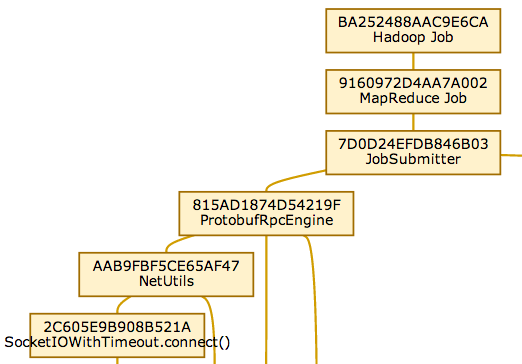
\includegraphics[width=0.6\textwidth]{figures/xtrace.png}
\caption{An snippet of X-Trace events logged during a Hadoop execution.}
\label{fig:xtrace}
\end{figure}

\subsection{Lower-level Tracing}
\label{ssec:low}
Tcpdump level tracing

\subsection{Tracing Results}
\label{ssec:results}
Non-dynamic results from tracing, e.g. tput graphs, sdn tests, etc.


